\documentclass{article}
\usepackage[left=1in,top=1in,right=1in,bottom=1in]{geometry}
\usepackage{time, amssymb, amsmath, amsthm, mathtools, witharrows, indentfirst}
\renewcommand{\qedsymbol}{\rule{0.7em}{0.7em}}
\newcommand{\pluseq}{\mathrel{+}=}
\newcommand{\timeseq}{\mathrel{*}=}
\newcommand{\minuseq}{\mathrel{-}=}
\usepackage[linesnumbered,ruled,vlined]{algorithm2e}
\usepackage{algpseudocode}
\setlength{\parindent}{0em}
\setlength{\parskip}{2em}
\usepackage{listings}
\usepackage{xcolor}
\usepackage{float}
\usepackage{ulem}

\definecolor{codegreen}{rgb}{0,0.6,0}
\definecolor{codegray}{rgb}{0.5,0.5,0.5}
\definecolor{codepurple}{rgb}{0.58,0,0.82}
\definecolor{backcolour}{rgb}{0.95,0.95,0.92}

\lstdefinestyle{mystyle}{
    backgroundcolor=\color{backcolour},   
    commentstyle=\color{codegreen},
    keywordstyle=\color{magenta},
    numberstyle=\tiny\color{codegray},
    stringstyle=\color{codepurple},
    basicstyle=\ttfamily\footnotesize,
    breakatwhitespace=false,         
    breaklines=true,                 
    captionpos=b,                    
    keepspaces=true,                 
    numbers=left,                    
    numbersep=5pt,                  
    showspaces=false,                
    showstringspaces=false,
    showtabs=false,                  
    tabsize=2
}

\lstset{style=mystyle}

\title{Engine Design Document for the AI Agent of Crossy Road}
\author{
  Yushan Weng\\
  \texttt{yweng@usc.edu}
  \and
  Shuwei Zhang\\
  \texttt{shuweiz@usc.edu}
  \and
  Veeraya Sawangsinudomchai\\
  \texttt{sawangsi@usc.edu}
  \and
  Wei Sun\\
  \texttt{wsun9780@usc.edu}
  \and
  Junzhe Liu \\
  \texttt{junzhel@usc.edu}
  \and
  Yilin Zhang \\
  \texttt{yzhang54@usc.edu}
}
\date{\today}

\usepackage{natbib}
\usepackage{graphicx}

\begin{document}

\maketitle

\tableofcontents

\section{Background and Overview}
\textit{Crossy Road} is an arcade video game released on 20 November 2014, developed and published by Hipster Whale. The game has been described as “endless Frogger”. The objective of \textit{Crossy Road} is to cross an endless highway or series of roads and avoid obstacles as far as possible without dying. The game we chose is a simplified browser version of the original \textit{Crossy Road}, where the obstacles are restricted to two types: the static tree that can block the movement, and the moving cars on the road that potentially can terminate the character.

The intuition of our neural network model is to train an agent that can play a simplified version of \textit{Crossy Road} game like a human being, even outperform than human. Because our model will train an agent to identify the incoming obstacles in the game, and make a decisions based on previous experiences to gain as much reward as it can, the ideal candidates for neural network architectures for our model are convolution network for computing vision, and reinforcement learning for reward functions. 

%\section{Context}


\section{Goals}
We learned that the current world record for the \textit{Crossy Road} developed by the Hipster Whale is \textbf{4,195}. Therefore, our expected our model at least get \textbf{1,000} to \textbf{2,000} score in the simplified version of \textit{Crossy Road}, and even better to get closer to the world record as possible. The expected result gives a detailed expectation for our model. First, we want the information captured by our convolution neural networks model to be as more accurate as possible. Second, we want the our reinforcement neural network can teach our agent to understand the game as good as a human being.

\section{Milestones}
\begin{center}
\begin{tabular}{ | c | c |} 
\hline
Week 2 & Proposed Project \\ 
\hline
Week 3 & Compared several approaches to set up the architecture of the project\\ 
\hline
Week 4 & Completed the framework for game agent\\ 
\hline
Week 5 & Set up a CNN for processing game image and collecting data\\ & Researched about how to combine RL and CNN \\ 
\hline
Week 6 - Week 8 & Built the model and started to tuning parameters \\ 
\hline
\end{tabular}
\end{center}

\section{Existing Solution}
So far, we have built a neural network model that are composed by three parts: computer vision, reinforcement learning, and automating the game playing. 

\subsection{Game Automation: Selenium API}
As we known, all the neural networks have to work on given input and will give output in number format. Therefore, we need to build a bridge between the game and neural networks that can pass the game as an input to game and operate game based on the output from neural networks. Because the game we work on is based on browser, we can take a advantage of Selenium API in python to implement this bridge. 

\subsubsection{Setup}
We work with Chrome browser because it has a complete console for debugging. Another thing we need to connect python and Chrome is a chromedriver. Then the setup process is as simple as below codes, where the driver is everything we need to operate Chrome through python.
\begin{lstlisting}[language=Python]
    driver = webdriver.Chrome()
\end{lstlisting}

We mainly use the \textit{driver} object to implement following operations:

\begin{itemize}
  \item Fix the browser GUI size and capture the game scene image as the input for CNN
  \begin{lstlisting}[language=Python]
driver.set_window_size(1200, 600)  
driver.save_screenshot(screen_shot_output)
    \end{lstlisting}
  \item Move the character in the game based on the output from model
  \begin{lstlisting}[language=Python]
driver.find_element_by_id("[next movement direction]").send_keys(Keys.[Direction])
    \end{lstlisting}
    \item Get the score achieved by the model
    \begin{lstlisting}[language=Python]
return driver.find_element_by_id('counter').text
    \end{lstlisting}
    \item Get if the game is over
    \begin{lstlisting}[language=Python]
return driver.find_element_by_id('retry').is_displayed()
    \end{lstlisting}
    \item Restart the game for timeless training
    \begin{lstlisting}[language=Python]
WebDriverWait(self._driver, 5).until(EC.element_to_be_clickable((By.ID, "retry"))).click()
# If the game is over, wait 5 seconds until the "retry" button shown up and available to be clicked
    \end{lstlisting}
    \item Shut down the game and the connection between Chrome and Python
    \begin{lstlisting}[language=Python]
driver.close()
    \end{lstlisting}
\end{itemize}



\subsection{Computer Vision: CNN}
In order to let the agent understand the game, we need to give our agent a pair of "eyes" to see the game, which is the computer vision part. This part is built on the convolution neural network architecture. In our implementation, we mainly used \textit{OpenCV} for image processing, and \textit{Sequential} models from \textit{keras} for building the CNN.

\subsubsection{Image Preprocessing}
With the captured image from the game, which represent the current state of the game,  we need to process it to a number form that be understand by our model. There are two requirements: 1. the image contains all necessary environmental information that influences the agent's next-step action decision, 2. the state should be as simple as possible to reduce computational complexity. 

Previously, we set the size of the image to $1200 \times 600$ pixels, which is so large that contains too much unnecessary information. After several approaches, we finally decided to chop the image to $80 \times 80$ pixels, which contains enough information representing the surrounding environment. This part is done by following code. 

\begin{lstlisting}[language=Python]
    image = image[200:400, 650:850]
    image = cv.resize(image, (80, 80))
\end{lstlisting}

Next, we observed that the color of the captured image is form \textbf{(R, G, B, a)}. Since the color does not help too much for edge detection, we transformed the image into grey mode. Moreover, we took the advantage of the edge detection in the \textit{OpenCV} to reduce the state space. The experimental result indicated that, compared to grayscale images, images with edge detection can reduce training time by $40\%$. The picture below visualizes this process. 

\begin{figure}[h]
\caption{Visualization of color transformation}
\centering
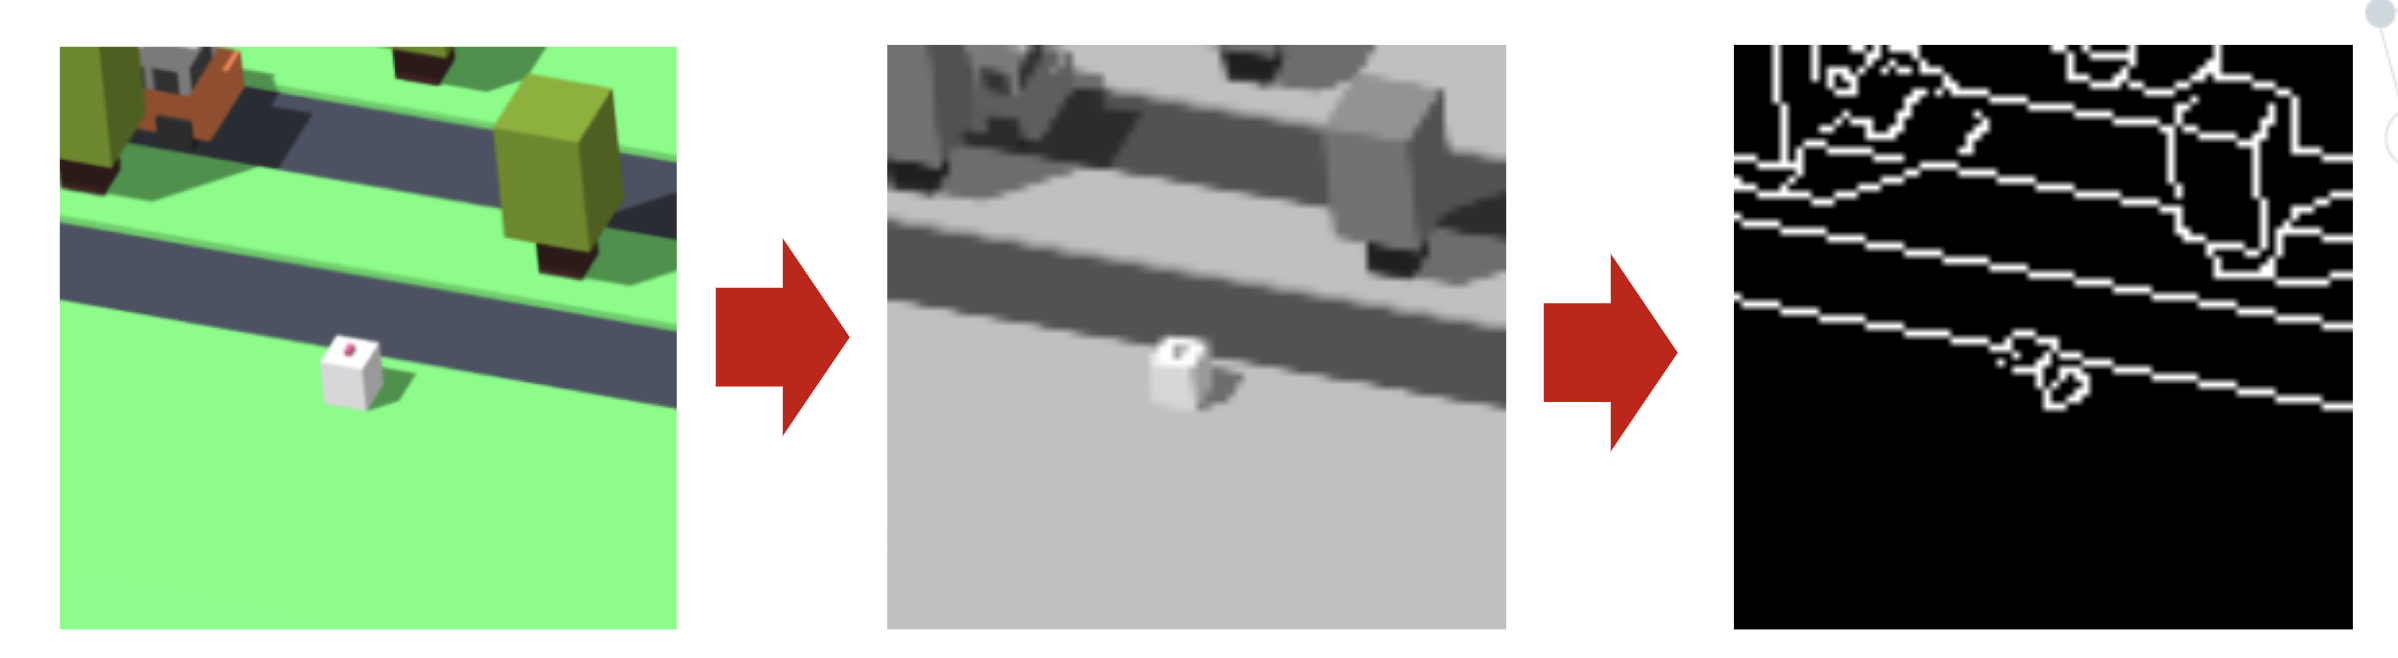
\includegraphics[width=0.5\textwidth]{color_transform_visualization.png}
\end{figure}

This process is done by following code.
\begin{lstlisting}[language=Python]
    image = cv.cvtColor(input_shot, cv.COLOR_BGR2GRAY)
    image = cv.Canny(image, threshold1=100, threshold2=200)
\end{lstlisting}

In conclusion, the whole preprocessing codes looks like below:
\begin{lstlisting}[language=Python]
def processing_image(self):
    input_shot = cv.imread(screen_shot_output)
    image = cv.cvtColor(input_shot, cv.COLOR_RGBA2GRAY)
    image = image[200:400, 650:850]
    image = cv.resize(image, (80, 80))
\end{lstlisting}


\subsubsection{Structure of Our CNN}
With the prepared input, now it's time to feed it into our CNN. Also, we have reduce the space of the image, we do not want miss any detail on the image, so we take 4 inputs to feed into CNN. Our CNN includes three convolutional layers and one flatten layer. In the last dense layer, we flatten into four neurons since we are considering only four operations of the game (move forward, move backward, move left, and move right). The output layer gives us the prediction of Q-value for each operation based on the input state. The picture below visualize the structure of our CNN model. 

\begin{figure}[h]
\caption{The Structure of CNN}
\centering
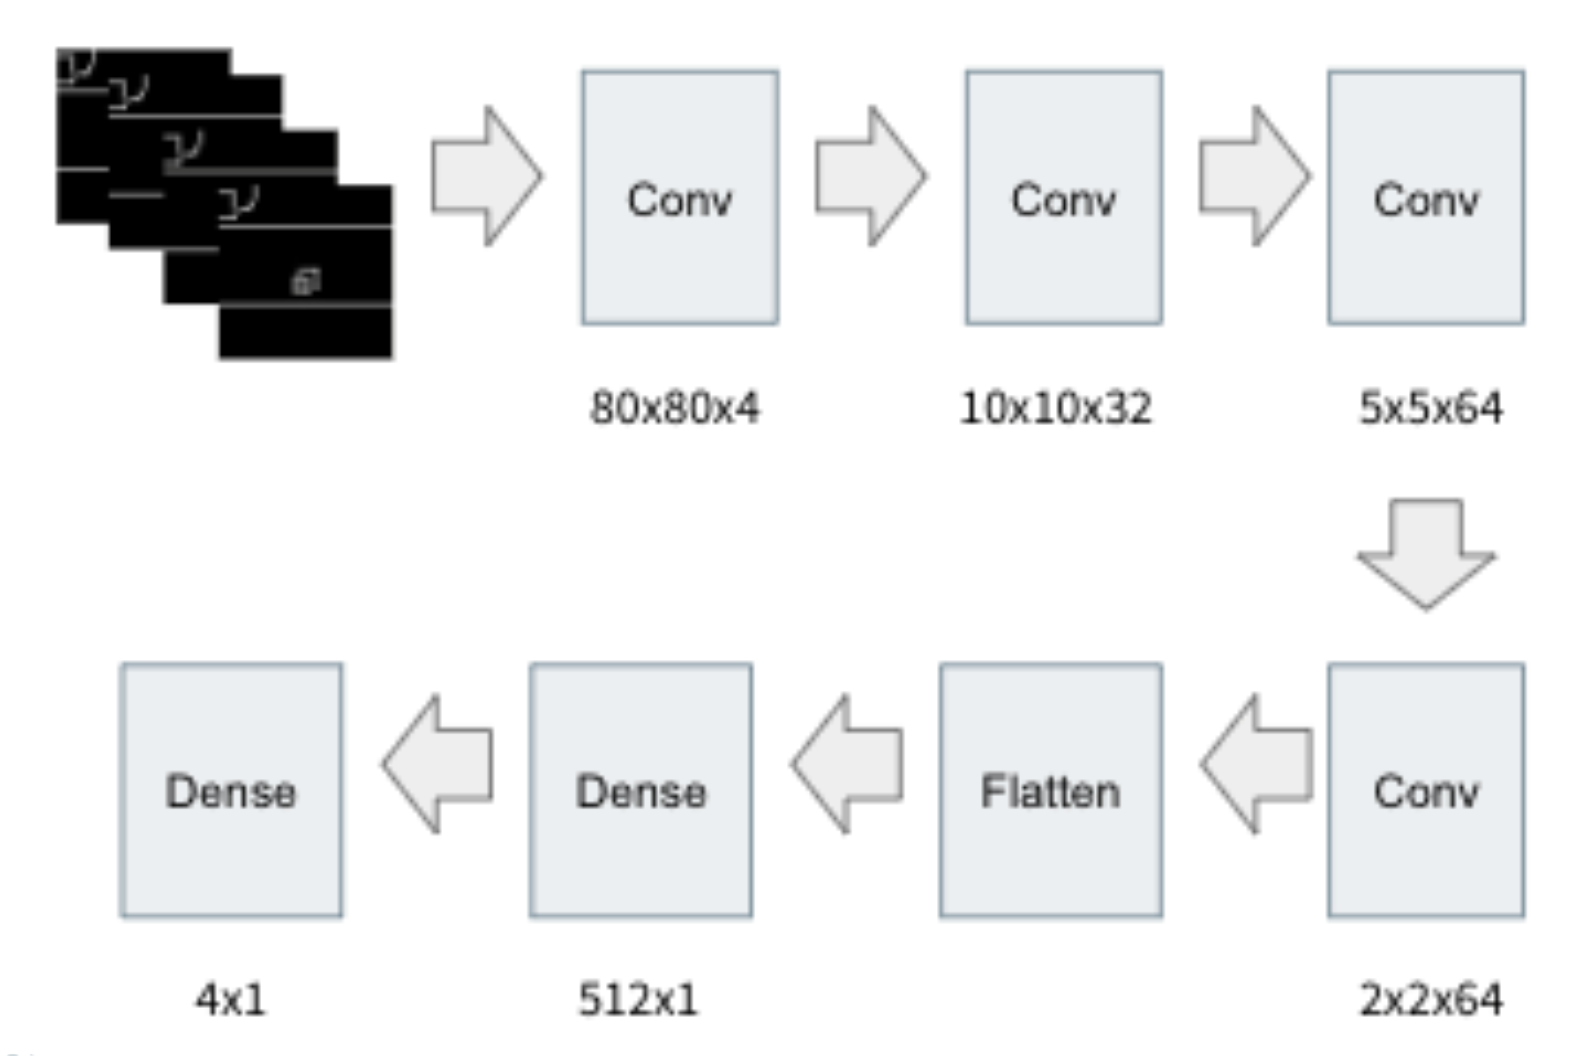
\includegraphics[width=0.5\textwidth]{CNN.png}
\end{figure}

The CNN is built by following code:
\begin{lstlisting}[language=Python]
def buildmodel():
    model = Sequential()
    # First layer
    model.add(Conv2D(32, (8, 8), padding='same', strides=(4, 4), input_shape=(img_cols, img_rows, img_channels)))
    model.add(MaxPooling2D(pool_size=(2, 2)))
    model.add(Activation('relu'))
    # Second layer
    model.add(Conv2D(64, (4, 4), strides=(2, 2), padding='same'))
    model.add(MaxPooling2D(pool_size=(2, 2)))
    model.add(Activation('relu'))
    # Third layer
    model.add(Conv2D(64, (3, 3), strides=(1, 1), padding='same'))
    model.add(MaxPooling2D(pool_size=(2, 2)))
    model.add(Activation('relu'))
    # Flatten layer
    model.add(Flatten())
    # Fully connect
    model.add(Dense(512))
    model.add(Activation('relu'))
    model.add(Dense(ACTIONS))
    adam = Adam(lr=LEARNING_RATE)
    model.compile(loss='mse', optimizer=adam)

    # Save the model file
    if not os.path.isfile(loss_file_path):
        model.save_weights(model_file_path)
    return model
\end{lstlisting}

\subsection{Reinforcement Learning: Reward Functions}
Learning about how to play the game is a learning process based on previous experience. Therefore, we decided to implement this process over reinforcement neural networks architecture. Specifically, we set a reward function. In the game, the agent will first observe the surrounding environment, and make a movement based on its observation. Then, the reward function will give a positive feedback if the decision update the score and a punishment if the decision caused gave over. 

\subsubsection{Combination of CNN and Bellman Equation}
Since our project looks at the long sequence of actions that can get the highest score, we need Bellman's equation to determine the long-term rewards.Therefore, to optimize, the Bellman equation can help us to find the optimal policy and value that can give us the better result.

$$V(S) = \max_{\alpha}(R(s, a) + \gamma\sum_{s'} P(s,a,s')V(s'))$$

As we mentioned before, the goal of the DQN is to choose a certain action(a) at state(s) in order to maximize the reward. Here, in our project, we combine the Convolution Neural Network with reinforcement learning techniques. We use CNN and Bellman’s Equation to estimate Q-value function required by Q-learning: the Neural Network serves as a non-linear approximator, which is optimized to minimize the difference between output and the target. In the next step, our agent will take the action with maximum Q-value.

The target, also named as Q-value iterative update function, is defined as follow:

\begin{equation}
    target_i = 
    \begin{cases}
    r_i & \textit{if game is terminated}\\
    r_i + \gamma max_{a^{'}}Q(s_{i + 1}, a', \theta) & \textit{if game is continued}
    \end{cases}
\end{equation}

where $max_{a^{'}}Q(s_{i + 1}, a', \theta)$ is the maximum Q-value achievable by any algorithm given the current condition(state $s$ and action $a$), which is the application of generalized Bellman’s Equation. $\gamma$, the discounted factor, is used to describe the influence of future reward. $\theta$ stands for the current policy, which is the current weights of the neural network.

\subsubsection{Certain Length Memory}

When the agent interacts with the environment, the sequence of experience can be highly correlated. In order to prevent the risk of getting swayed, we applied experience replay in our project. We sampled a minibatch of size of 32 from the replay memory we set up when initialization. Also, we set a fixed length for the memory to refresh the replay space and ensure timeliness.

\subsubsection{Observe, Explore, and Train}
To have enough data for training, our Deep Q-learning algorithm was designed by two phases: Observation and Train. In the Observation phase, we need to choose an action $(a)$ randomly. Considering the balance between exploitation and exploration, we deployed the Epsilon-greedy strategy to random choose an action a. The agent will take action $(a)$ and observe reward $(r)$ and next state $(s’)$. With several experiments, we find that 10,000 is a reasonable steps, in which the agent can gain enough experience without over training. The tuple for the transaction (s, a, r, s’, is\_dead) was stored in the experience replay memory. 

In the training phase, we sample a random minibatch of 32 transitions from the experience replay memory. We enumerate the batch and update the expected state-action values using the Bellman’s Equation. The whole Q-network was updated by minimizing the loss with Adaptive Moment Estimation optimizer.

In conclusion, here is a pseudo code demonstrating how the DQN agent is built. 

\begin{algorithm}
train\_round = 0\;
memory = Deque()\;
\While(Timeless training){True} {
    state = game screen capture\;
    \If{train\_round $\leq$ 10,000} {
        action = random(forward, backward, left, right)\;
    }\Else {
        action = model.predict(state)\;
    }
    
    nextMove(action)\;
    new\_state = game screen capture\;
    is\_dead = if game is over\;
    game\_score = game score\;
    reward = rewardFunction(action, new\_state, is\_dead, game\_score)\;
    memory.pushRight((state, new\_state, reward, is\_dead))\;
    \If{train\_round $>$ 10,000}{
        mini\_batch = sample(memory, 32)\;
        Optimize the model by train on mini\_batch\;
    }
    train\_round++\;
}
\end{algorithm}

\section{Alternative Solution}

According to the results from the initial implementation, we noticed that there are two potential variables that affect the accuracy of our model: obstacles detection and the design of the reinforcement learning feature. Therefore, we proposed several alternative solutions.

\subsection{Accuracy of Object Detection of CNN}
We realized that the top priority of our model is to detect the obstacles in the game. We observed that the current view of the game is from the top left corner, which has negative impact to our model. Therefore, we decide to lower the difficulty our model and transfer the original view to the top view. 

\begin{figure}[h]
    \caption{Top view Image Processing}
    \centering
    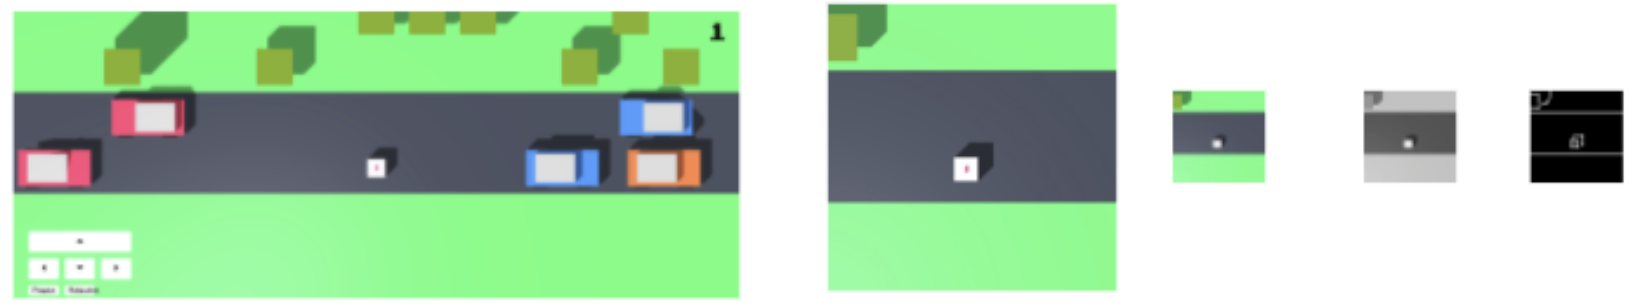
\includegraphics[width=0.5\textwidth]{topAngel.png}
\end{figure}

Even if the agent seems to perform better with the lower difficulty, there are several issues occurring in the training process. The first problem is the high variance of $Q$ value, and it makes the bellman equation too weak since the reward is too small from the biggest $Q$ value. It does not make any changes in the reward function. The second challenge is the complexity of the image input. It is not only a 3D game, but also the shadow as well. \par 

To solve the high Q value, we normalize the image input by the code in below. 
\begin{lstlisting}[language=Python]
def processing_image():
    img_64 = self.game.driver.find_element_by_id('imgURL').text
    screen = np.array(Image.open(BytesIO(base64.b64decode(img_64))))
    img = cv.cvtColor(screen, cv.COLOR_RGBA2GRAY)
    img = img[100:800, 850:1550]
    img = cv.resize(img, (80, 80))
    img = cv.Canny(img, threshold1=100, threshold2=200)
    # Normalize the image input
    img = (img - img.mean()) / (img.std() + 1e-8)
    return img
\end{lstlisting}

Next, we added the following code in the training process to normalize the Q value.
\begin{lstlisting}[language=Python]
temp_next_state = model.predict(state_t1)
# Normalize q value in list to range between 0 and 1
normal_target_next_state = np.linalg.norm(temp_next_state)
normal_next_array = temp_next_state / normal_target_next_state
Q_sa = normal_next_array   
\end{lstlisting}

According to the result, we restricted the Q value between 0 and 1. \par 

Moreover, although we introduced the edge detection from OpenCV, we noticed that shadow of objects increased the complexity of the input state, like in the figure 4.

\begin{figure}[h]
    \caption{Example of the edges of shadow}
    \centering
    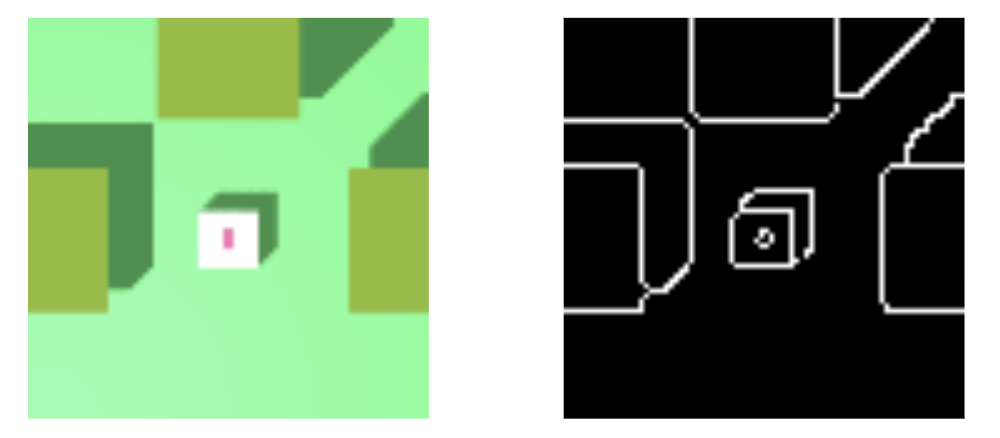
\includegraphics[width=0.5\textwidth]{ShadowEdge.png}
\end{figure}

Since the only thing that we consider is the obstacles in game, which are cars, trucks, and trees, we can reduce the complexity of the game by changing the background color to black, like in figure 5. This solution also solves the shadow problem from the game as well. \par 

\begin{figure}[h]
    \caption{Example of game view in black background}
    \centering
    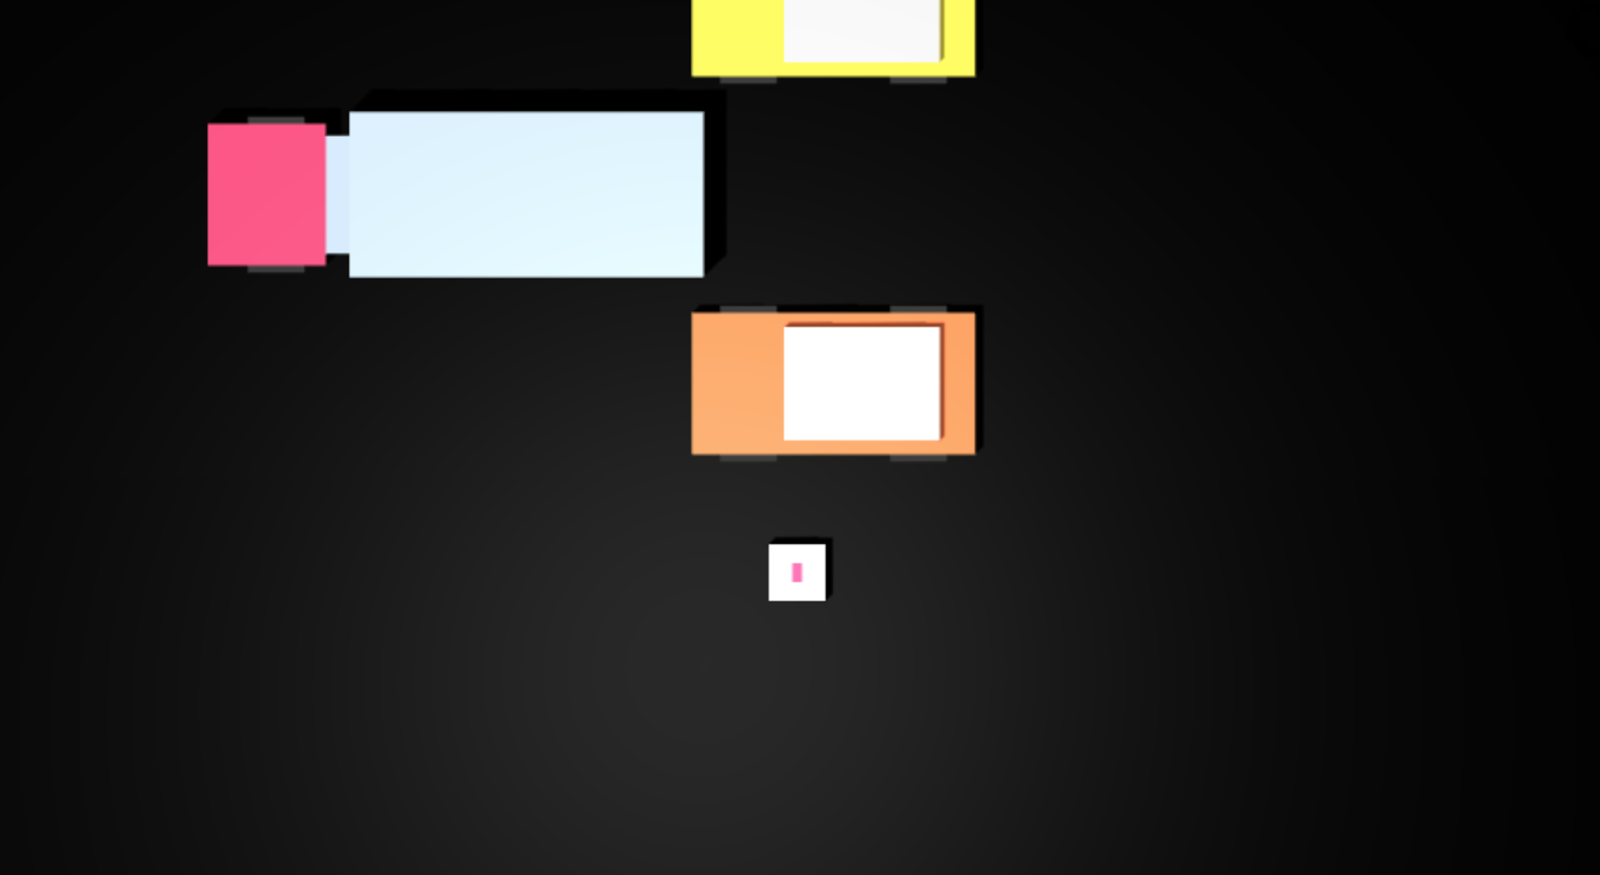
\includegraphics[width=0.5\textwidth]{blackground.png}
\end{figure}

As a result after training our agent more than 5000 episodes with the new environment of the game, as in figure 6, the agent seems to not be making any improvement. We notice that the agent cannot avoid the vehicles at all. \par 

\begin{figure}[H]
    \caption{Result with Black Background}
    \centering
    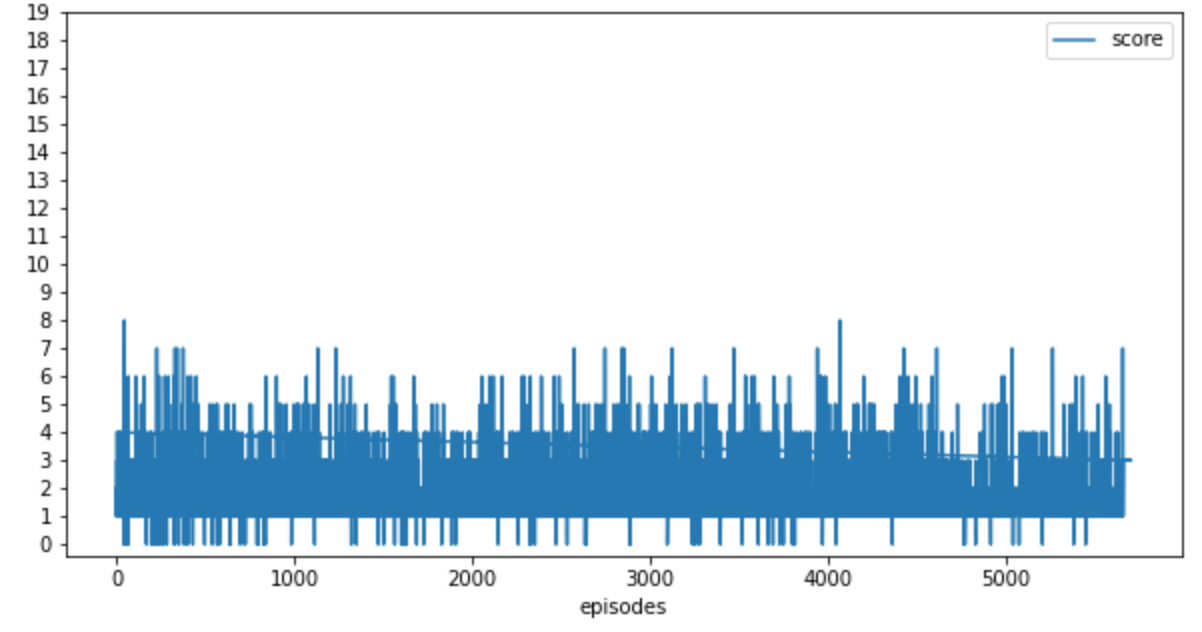
\includegraphics[width=0.5\textwidth]{result_black_background.png}
\end{figure}

\subsection{New Action}
We noticed that people will hesitate to consider for next movement while they are playing the game. The next attempt is rather than considering only four actions, which are move forward, move left, move right, and move backward, we will consider five actions by adding stay still for our agent. We notice that “STAY” is more important in the game since the agent needs to wait until the vehicle is passed, and the best action based on this scenario is to choose the stay action and wait. Therefore, “STAY” action has been implemented for the next attempt. Below is the mapping value that we use to map the action with the number.

\begin{center}
    \begin{tabular}{ | c | c |} 
        \hline
        Action & Key \\ 
        \hline
        Stay & 0\\ 
        \hline
        Forward & 1\\ 
        \hline
        Backward & 2 \\ 
        \hline
        Left & 3 \\
        \hline
        Right & 4 \\ 
        \hline
    \end{tabular}   
\end{center}

\subsection{New Design of the Model}
\subsubsection{Prepartion}
To construct every new model, this process takes some amount of time to build a new code, so the idea of implementing Stable Baselines comes in. Stable Baselines library is introduced by the openAI team, which consists of the set of improvement implementations on Reinforcement learning in openAI such as DQN, A2C, PPO, etc. \par 

Since Stable baselines is the RL tool on openAI, and openAI will work on the environment that follows the structure on openAI Gym. Therefore, a custom environment has been built by constructing the openAI Gym structure with following code. 

\begin{lstlisting}[language = Python]
class ChromeCrossyRoadEnv(gy.Env):
    def __int__(self):
        self.game = CrossyRoadGame()
        n_action = 5
        self.action_space = spaces.Discrete(n_actions)
        self.observation_space = spaces.Box(low=0, high=255, shape=(80, 80), dtype=np.uint8)
        self.gametime_reward = 0.1
        self.gameOver_penalty = -1
        self.current_frame = self.observation_space.low
        self._action_set = [0, 1, 2, 3, 4]

        self.game_score = self.game.get_score()
\end{lstlisting}

\subsubsection{New Approaction 1: Deep Q-Network (DQN) with Prioritized Experience Replay (PER)}
The biggest problem of the vanilla Deep Q-network is uniformly sampling the experience from a replay memory or buffer, but some experiences are more important than others. To feed the important experience into the neural network, we try to bring the idea of Prioritized Experience Replay in our model. With PER, it will weigh the samples so that the important experience will be drawn more often on the training process.  The main goal of DQN is to find a policy that maps a given state to an action that can maximize the expected reward of the agent. To be prioritized the experience, the absolute TD error is used.

$$\delta_i = r_t + \gamma \cdot \max_{a \in A} (Q_{\theta^-}(s_{t + 1}, a)) - Q_{\theta}(s_t, a_t)$$

TD error is used as the absolute error $|\delta_i|$ as the absolute, so the negative error and the positive error will be the same in this method. In order to work with the DQN, we assign $|\delta_i|$ into the samples, which is $(s_t,a_t,r_t,s_{t+1},|\delta_i|)$. In order to update the absolute TD errors, we do not need to update all values. We do need to update $|\delta_i|$ term for the item that is actually sampled during the mini batch gradient updates. For a minibatch size of 32, each gradient update will change the priorities of only 32 samples in the replay buffer, and leave most of the item alone with touching. \par 

There are two ways to calculate the priorities score, denoted as $p_i$:
\paragraph{A Rank Based Method:}
$$p_i = \frac{1}{\text{rank}(i)}$$
Where $\text{rank}(i)$ is the rank of transition from sorting the replay memory based on $|\delta_i|$.

\paragraph{A Proportional Variant:}
$$p_i = |\delta_i| + \epsilon$$

Where $\epsilon$ is a small constant that prevent the transition from zero probability of being drawn. \par 

Either two method above, we will be able to get a probabilistic distribution for sampling by calculating the equation below:
$$P(i) = \frac{p_i^{\alpha}}{\sum_{k}p_k^{\alpha}}$$

Where $\alpha$ determines the prioritized level in the memory. If $\alpha$ is close to 0, then there is no prioritization. If $\alpha$ is close to 1, then there is prioritization in the sampling.

\paragraph{Implementation}
Below is the pseduo-code of the DQN with PER. \par 

\begin{algorithm}[H]
    \caption{DQN with experience replay}
    Initialize replay memory $D$ to capacity $N$ \;
    Initialize action-value function $Q$ with random weights $\theta$\;
    Initialize target action-value function $\hat{Q}$ with weights $\theta^{-} = \theta$\;
    \For{episode = 1}
    {
        Initialize sequence $s_1 = {x_1}$ and preprocessed sequence $\phi_1 = \phi(s_1)$\;
        \For{t = 1}
        {
            \If{Observation Stage}
            {
                With probability $\varepsilon$ select a random action $a_t$\;
            } \Else
            {
                $a_t = \text{argmax}_a(Q(\phi(s_t), a; \theta))$\;
            }

            Execute action $a_t$ in the game and observe reward $r_t$ and game state $s_{t+1}$\;
            Store transition $(\phi_t, a_t, r_t, \phi_{t + 1})$ in $D$\;
            Sample random minibatch of transition $(\phi_j, a_j, r_j, \phi_{j + 1})$ from $D$\;
            \If{Episode terminates at step $j + 1$}
            {
                $r_j$\;
            } \Else 
            {
                $r_j + \gamma \max_{a'}(\hat{Q}(\phi_{j + 1}, a'; \theta^-))$
            }
            Perform a gradient descent step on $(y_j - Q(\phi_{i}, a_j; \theta))^2$ with respect to the network parameter $\theta$\;
            $\hat{Q} = Q$\;
        }
    }
\end{algorithm}

With the openAI package and previously set baselines environment, the actually implementation is as simple as the code in below
\begin{lstlisting}[language = Python]
env = gym.make('ChromeCrossyRoad-v0')
model = DQN("MlpPolicy", env, learning_rate=0.0001, gamma=0.7, batch_size=1024, prioritized_replay=True, verbose=1, tensorboard_log="./log/dqn_crossy_road_tensorboard/")
model.learn(total_timesteps=30000)
model.save("../model/DQN")
env.close()
\end{lstlisting}

\subsubsection{New Approaction 2: Advantage Actor Critic (A2C)}

To recall, we use the value based methods to train our agent where we learn a value function by mapping the state and action pair to a value. We will select the best action by selecting the action that can give the biggest Q value. But there are several methods of reinforcement learning that exist in this world, which are Policy based methods or  Reinforcement with Policy Gradients. Rather using the value function, we can directly optimize the policy. This method is trying to find a good score function to compute how good a policy is. \par 

However, these two methods on reinforcement learning have the biggest drawback; therefore, instead of selecting either value base methods or policy based methods, we do use two methods to train our agent. This is how A2C comes in. \par 

The biggest problem of the Policy Gradients is that we need to wait until the end of the episode in order to calculate the score, which is known as Monte Carlo. Especially in the Crossy Road game, the chicken can be alive for a long time, but it does mean that we can earn a high score from the game.
It may end with the very high reward. But in fact, our agent got stuck with the obstacle, like in figure 7; therefore, we decided to implement A2C to solve that problem. \par

\begin{figure}[h]
    \caption{Struggle with tree}
    \centering
    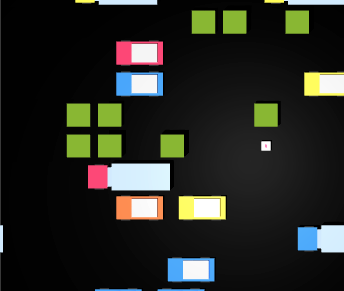
\includegraphics[width=0.5\textwidth]{obstacles_trapped.png}
\end{figure}

A2C is the hybrid method that uses both value based method and policy based method. It use two neural network as below:
\begin{itemize}
\item A Critic will measure how good the taken action is(value-based)
\item An Action will measure how well our agent performs(policy-based)
\end{itemize}

Instead of waiting until the end of the episode to calculate the reward, we do update them after each time step. Since we update the 
$$\text{Policy Update: } \Delta \theta = \alpha \cdot \nabla_{\theta} (\log(\pi (S_t, A_t, \theta))) \cdot R(t)$$
$$\Downarrow$$
$$\text{New update: } \Delta \theta = \alpha \cdot \nabla_{\theta} (\log(\pi (S_t, A_t, \theta))) \cdot Q(S_t, A_t)$$

Since we update the weight in each time step, the total reward(R(t)) from each episode cannot be used in this model. The total reward R(t) is replaced by the function value, which is the idea of value based method. This is how the value based method comes in the A2C. \par 

As we mention, A2C needs two neural networks to implement and need to run parallel. The first one is the Actor Neural Network. It starts randomly performing the action, and then the Critic Neural Network will observe and provide the feedback from the action that is taken inside the game in terms of loss. Based on the feedback from the Critic neural network, the Actor neural network will be able to update the policy and get better results. Not only the Actor, but also the Critic as well, will update the feedback policy in order to give useful feedback to the Actor. \par

\begin{figure}[H]
    \caption{A2C Architecture}
    \centering
    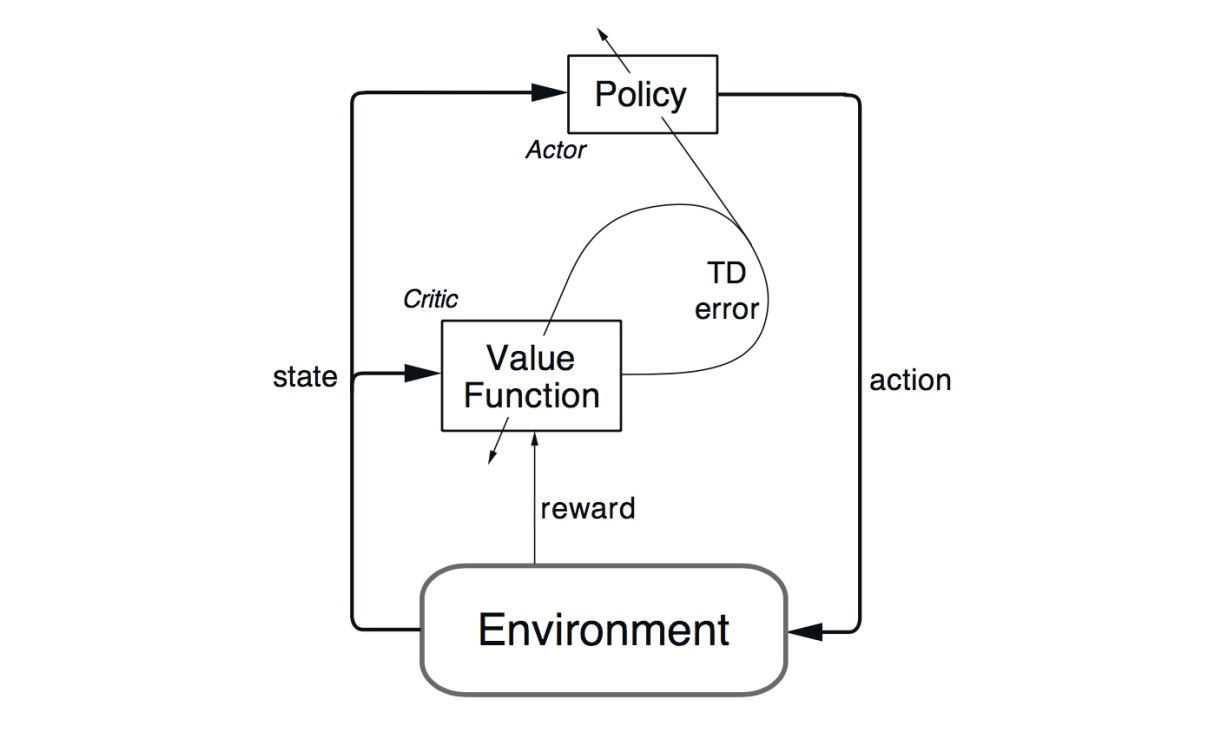
\includegraphics[width=0.5\textwidth]{A2C_Arch.png}
\end{figure}

Since we have two neural networks for the Actor and the Critic,  we need to estimate both networks. \par 

$$\text{Actor: A policy function, controls how our agent acts: } \pi(s, a, \theta)$$
$$\text{Critic: A value function, measures how good these actions are: } \hat{q}(s, a, w)$$

We need to train both networks simultaneously, which means that we need two sets of the weight for each network. \par

\begin{figure}[H]
    \centering
    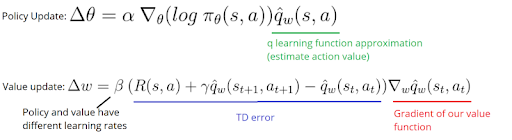
\includegraphics[width=0.5\textwidth]{A2C_eq.png}
\end{figure}

For each input, the Critic will observe and compute the $Q$ value after taking the action on the state, and the Actor will update the policy parameter(weight) by using the $Q$ value that the Critic. \par 

$$\Delta \theta = \alpha \cdot \nabla_{\theta} (\log{\pi (S_t, A_t, \theta)}) \cdot \hat{q}_w(S_t, A_t)$$

After the Actor updates the weight, it will produce the next action to take with the next state, and the Critic then will update its values parameter. \par 

$$\Delta w = \beta(R(s, a) + \gamma \hat{q}_w(s_{t + 1}, a_{t + 1}) - \hat{q}_w(s_t, a_t)) \nabla_w \hat{q}_w(s_t, a_t)$$

\paragraph{Implementation}
Below is the pseduo-code of the A2C. \par 
\begin{algorithm}[H]
    \caption{Advantage Actor Critic (A2C)}
    Initialize parameters $s, \theta, w$ and learning rates $\alpha_{\theta}, \alpha_{w}$; sample $a \sim \pi_{\theta}(a|s)$\;
    \For{$t: 1 \rightarrow T$}
    {
        Sample reward $r_t \sim R(s, a)$ and next state $s' \sim P(s'|s, a)$\;
        Sample the next action $a' \sim \pi_{\theta}(a'|s')$\;
        Update the policy parameters: $\theta \leftarrow \theta + \alpha_{\theta} Q_w(s, a) \nabla_{\theta} \log{\pi_{\theta} (a|s)}$\;
        Compute the correction (TD-error) for action-value at time $t$: $\delta_t  = r_t + \gamma Q_w(s', a') - Q_w(s, a)$\;
        Update the parameters of $Q$ function: $w = w + \alpha_w \delta_t \nabla_w Q_w(s, a)$
        $a = a'$\;
        $s = s'$\;
    }
\end{algorithm}

With the openAI package and previously set baselines environment, the actually implementation is as simple as the code in below
\begin{lstlisting}[language = Python]
env = gym.make('ChromeCrossyRoad-v0')
model = A2C("MlpPolicy", env, learning_rate=0.0001, gamma=0.7, batch_size=1024, verbose=1, tensorboard_log="./a2c_crossy_road_tensorboard/")
model.learn(total_timesteps=30000)
model.save("../model/A2C")
env.close()
\end{lstlisting}

\subsubsection{New Approaction 3: Proximal Policy Optimization (PPO)}
In 2017, the openAI team introduced Proximal Policy Optimization or PPO, which is the improvement of Advantage Actor Critic(A2C). The implementation of PPO is the same as A2C, but the big difference is the way to estimate the policy gradient. PPO used the ratio between the new and old policy that is scaled by advantages instead of using the logarithm of the new policy.

$$L^{CPI}(\theta) = \hat{\mathbb{E}}_t [\frac{\pi_{\theta} (a_t | s_t)}{\pi_{\theta_{\text{odd}} (a_t | s_t)}} \hat{A_t}] = \hat{\mathbb{E}}_t[r_t(\theta)\hat{A}_t]$$

\paragraph{Implementation}
Below is the pseduo-code of the Proximal Policy Optimization \par 

\begin{algorithm}[H]
    \caption{PPO-Clip}
    \KwIn{Initial policy parameters $\theta_0$, initial value function parameter $\phi_0$}

    \For{$k: 1 \rightarrow \infty$}
    {
        Collect set of trajectories $\mathcal{D}_k = \{\tau_i\}$ by running policy $\pi_k = \pi(\theta_k)$ in the environment\;
        Compute rewards-to-go $\hat{R}_t$\;
        Compute advantage estimates, $\hat{A}_t$ based on the current value function $V_{\phi_k}$\;
        Update the policy by maximizing the PPO-Clip objective: 
        $\theta_{k + 1} = \arg \max_{\theta} \frac{1}{|\mathcal{D}_k|T} 
        \sum_{\tau \in \mathcal{D}_k}
        \sum_{t = 0}^T \min (\frac{\pi_{\theta} (a_t | s_t)}{\pi_{\theta_k} (a_t | s_t)} A^{\pi_{\theta_k}} (s_t, a_t), g(\epsilon, A^{\pi_{\theta_k}} (s_t, a_t)))$ \;
        Fit value function by regression on mean-squared error: 
        $\phi_{k + 1} = \arg \min_{\phi} \frac{1}{|\mathcal{D}_k|T}  \sum_{\tau \in \mathcal{D}_k}
        \sum_{t = 0}^T (V_{\phi}(s_t) - \hat{R}_t)^2$\;
    }
\end{algorithm}

With the openAI package and previously set baselines environment, the actually implementation is as simple as the code in below
\begin{lstlisting}[language = Python]
env = gym.make('ChromeCrossyRoad-v0')
model = PPO("MlpPolicy", env, learning_rate=0.0001, gamma=0.7, batch_size=1024, verbose=1, tensorboard_log ="./log/ppo_crossy_road_tensorboard/")
model.learn(total_timesteps=30000)
model.save("../model/ppo")
env.close()
\end{lstlisting}

\subsubsection{Model Selection}
As we mentioned before, we are encountering limitations on the training process since our game environment does not work well with Google colab. It takes some amount of time to train each model and check the result. Therefore, we do some model selection by training only 30,000 timesteps with the same set of parameters and keep monitoring the result for DQN, A2C, and PPO so that we can focus on training only one model and tune hyperparameter. During the training process, PPO seems to perform better than the other two since this agent can avoid the tree, which is the most challenging that we were encountering for a long time, while the other two models still get stuck within the tree. Now we will mainly focus on training our agent on the PPO model. \par 

After tuning multiple times, below is the hyperparameter that we set in order to achieve the high score. \par 

\begin{center}
    \begin{tabular}{ | c | c |} 
        \hline
        Action State & Reward \\ 
        \hline
        Stay & -10\\ 
        \hline
        Forward & +7\\ 
        \hline
        Backward & -200 \\ 
        \hline
        Left & 0 \\
        \hline
        Right & 0 \\ 
        \hline
    \end{tabular}   
\end{center}

\section{Experiments and Results}
We noticed that there are variables that potentially can affect the performance of our model: the accuracy of the CNN model and the setting of our reward functions. Therefore, we divided into two branches that each branch will check one of the variables. 

\subsection{Reward Function Setting}
We checked three different sets of reward functions

\subsubsection{The control group}
For the control agent, we set all the rewards for different actions to be the same. And the reward was set to -1 if the game crashed.

\begin{center}
    \begin{tabular}{ | c | c| c | } 
    \hline
    Action State & Reward\\ 
    \hline
    Forward & 0.1\\ 
    \hline
    Backward & 0.1\\ 
    \hline
    Left & 0.1\\ 
    \hline
    Right & 0.1\\ 
    \hline
    Game Over & -1\\ 
    \hline
    \end{tabular}
\end{center}

Here is the result of the control group
\begin{figure}[h]
\caption{Visualization of color transformation}
\centering
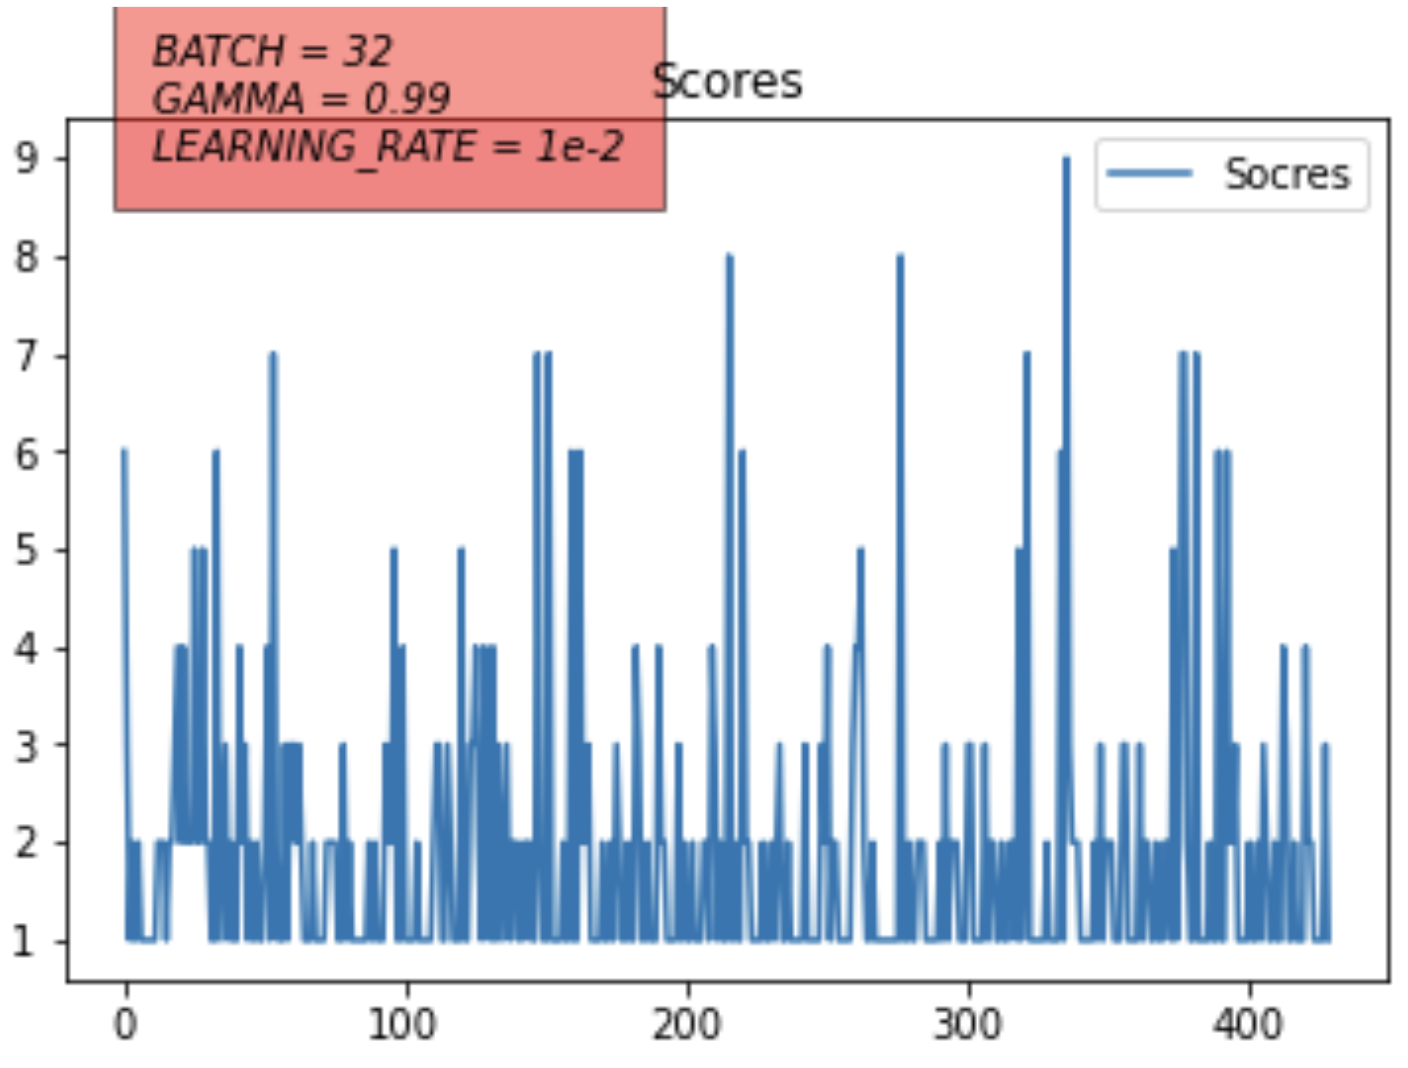
\includegraphics[width=0.5\textwidth]{ControlAgent.png}
\end{figure}

\subsubsection{First Attempt}
Next, we set the reward to be more reasonable. Give more reward if the agent goes forward. At the same time, give a negative reward on moving backward since we don’t want it to move backward. The reward for left and right is smaller than forward because we’d like to encourage the agent to move forward instead of doing a left-to-right jump.

\begin{center}
\begin{tabular}{ | c | c| c | } 
\hline
Action State & Reward\\ 
\hline
Forward & 1\\ 
\hline
Backward & -1\\ 
\hline
Left & 0.1\\ 
\hline
Right & 0.1\\ 
\hline
Game Over & -10\\ 
\hline
\end{tabular}
\end{center}

Based on the experiment we did on Agent 1, we found that we need the agent to go backward sometimes. For example, there are some “traps” in the game. We could not get a better result when the agent was trapped.

\begin{figure}[h]
\caption{Trap in the game}
\centering
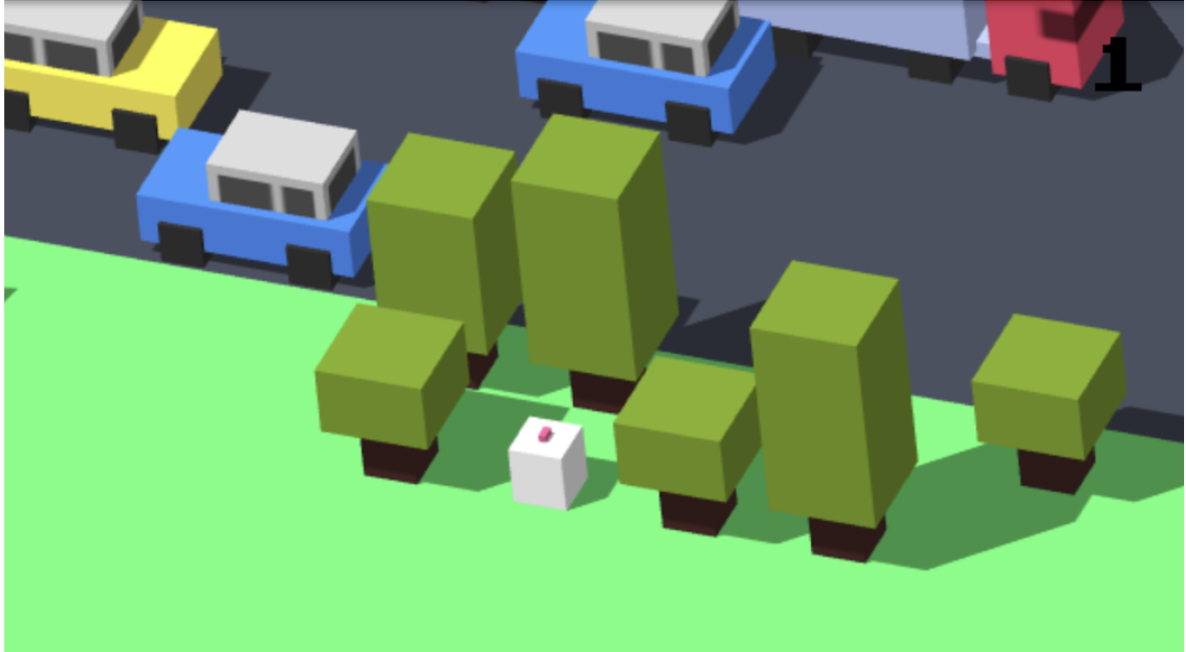
\includegraphics[width=0.5\textwidth]{trap.png}
\end{figure}

\subsubsection{Second Attempt}
The previous agent tends to be stuck at the same point in the last experiment. Thus, we set the second agent as below, which we do not punish the agent for backward movement since it can be necessary in some scenarios:

\begin{center}
\begin{tabular}{ | c | c| c | } 
\hline
Action State & Reward\\ 
\hline
Forward & 1\\ 
\hline
Backward & 0\\ 
\hline
Left & 0.1\\ 
\hline
Right & 0.1\\ 
\hline
Game Over & -10\\ 
\hline
\end{tabular}
\end{center}

Here is the result of the second group. According to the figure below, it is clear that the result was not improved too much. 


\begin{figure}[h]
\caption{The result of the Second Agent}
\centering
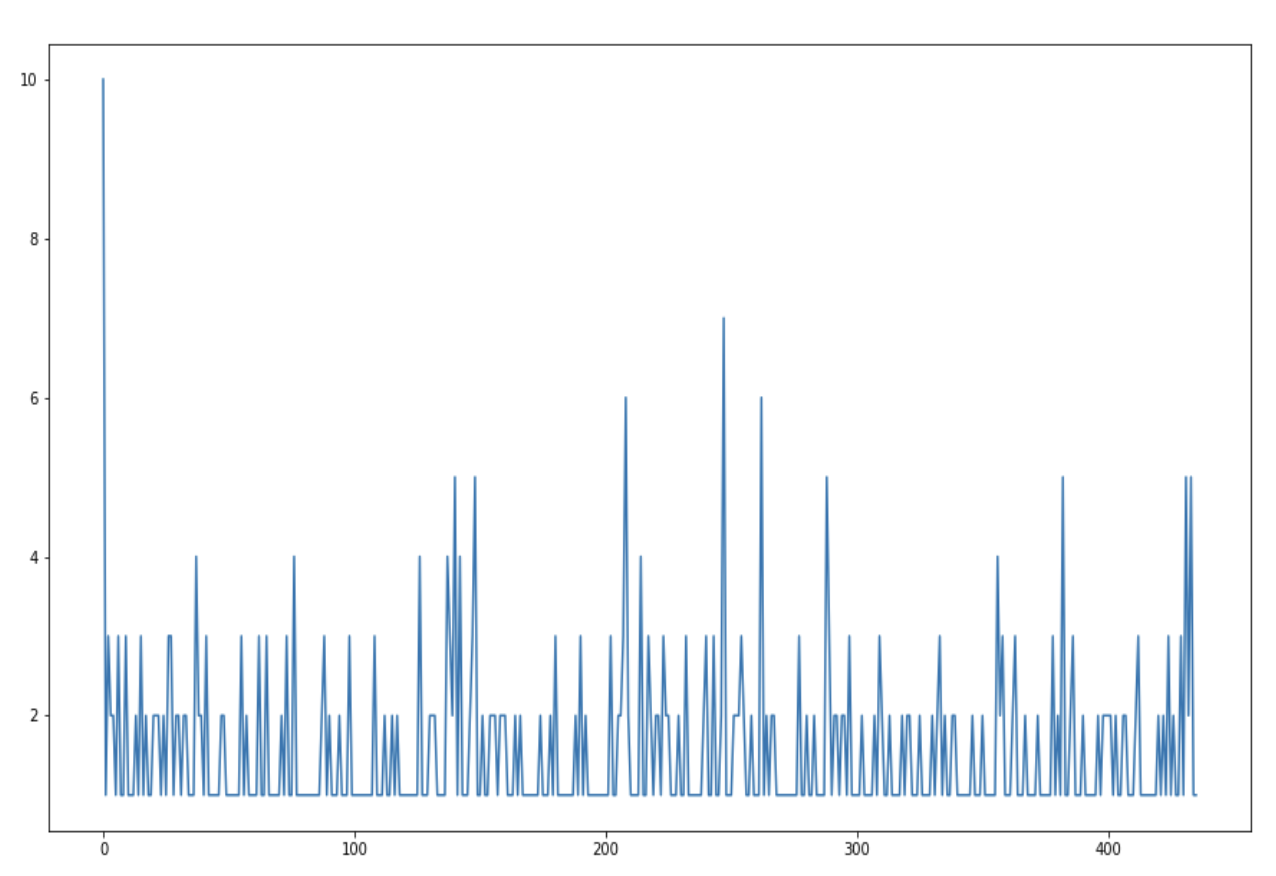
\includegraphics[width=0.5\textwidth]{SecondAgent.png}
\end{figure}

\subsubsection{Third Agent}
For the third agent, we designed it to build some relationship between score and reward. Thus, we set the reward to be changes of score.


\begin{center}
\begin{tabular}{ | c | c| c | } 
\hline
Action State & Reward\\ 
\hline
Forward & New\_Score - Old\_Score\\ 
\hline
Backward & New\_Score - Old\_Score\\ 
\hline
Left & New\_Score - Old\_Score\\ 
\hline
Right & New\_Score - Old\_Score\\ 
\hline
Game Over & -10\\ 
\hline
\end{tabular}
\end{center}

We can tell from the result of Agent 3 that the improvement in score is limited. However, the variance of the score is much lower. 

\begin{figure}[H]
\caption{The Result of the Third Agent}
\centering
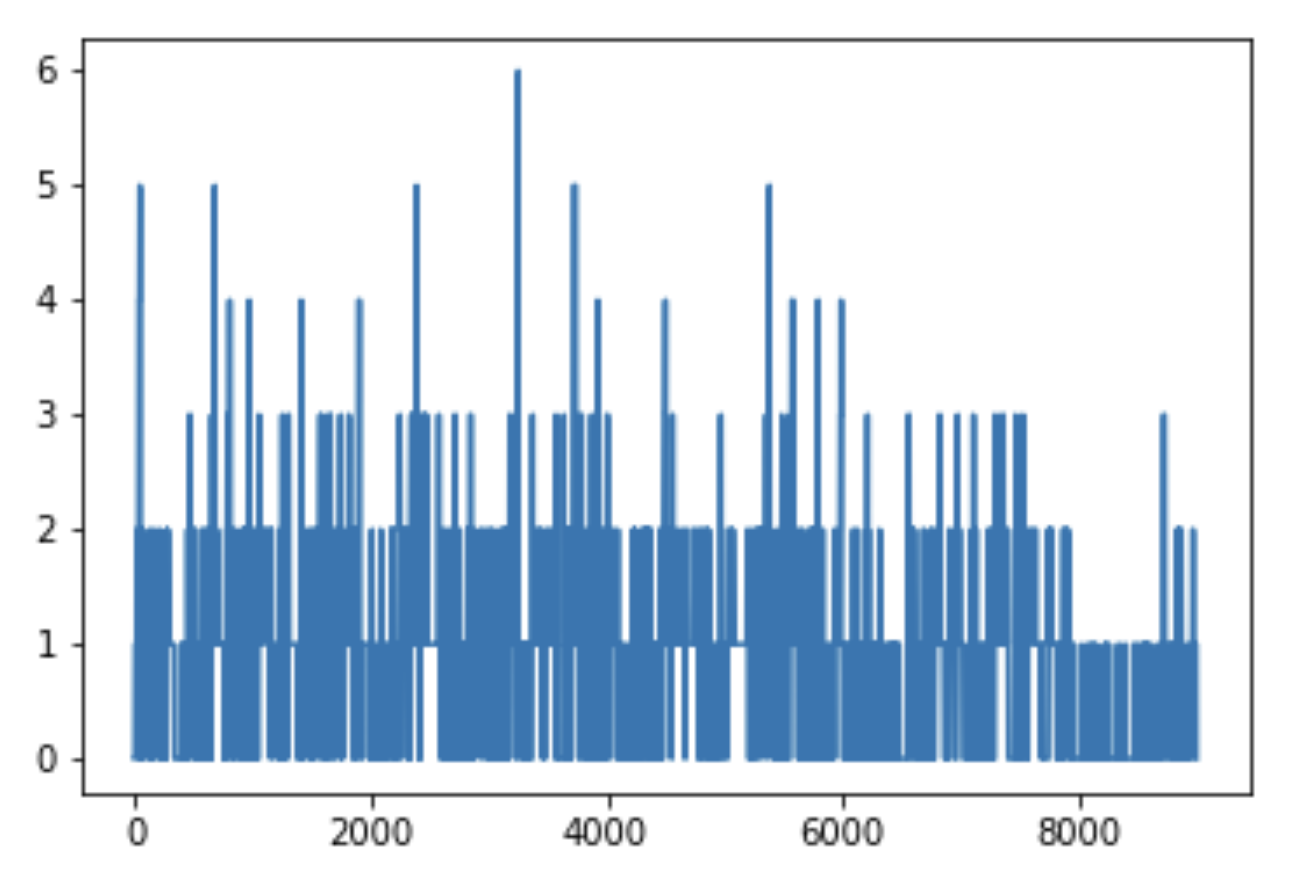
\includegraphics[width=0.5\textwidth]{ThirdAgent.png}
\end{figure}

% \subsubsection{Conclusion}
% From testing these agents with different reward functions, we have not be able to find a clear direction for the parameter tuning of the reward functions. However, we noticed that the third agent indicated that there can be relationship between reward function and the changes in score. There is another problem is that rounds of game played by each agent is quite low, which is caused by the limitation of computing power of our devices. Hopeful, in the next steps, we can find some ways to improve our computing power, and be able to find a clear direction for parameter tuning with enough rounds of game playing.

% \subsection{Image Processing Improvement}
% We also noticed that there may be some improvements that we can do on the image processing parts. We observed that the current viewpoint in the game scene is on the top back left corner. The problem is with this region we cannot capture all information that needs to be used for our model in this view of the game. For example, we are unable to see the left of the character especially when there are obstacles on the left diagonal originated from the character.

% \subsubsection{Potential Solution}
% Our current solution is kind of brutal. We did a hard coding hack to the base code, and changed the view to the top right above the character. The result game scene looks like the figure below.

% \begin{figure}[h]
% \caption{Top view Image Processing}
% \centering
% 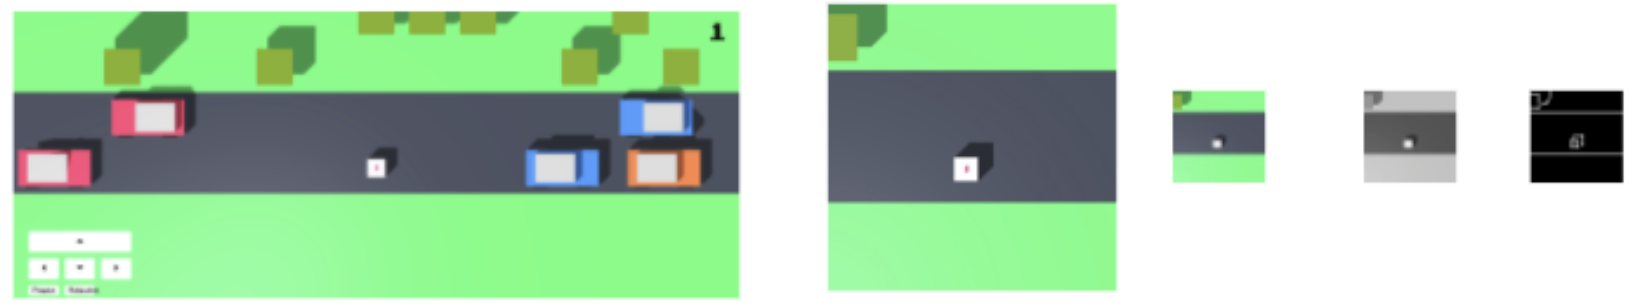
\includegraphics[width=0.5\textwidth]{topAngel.png}
% \end{figure}

% With this different view, we trained another agent with the reward function setting in the following table:

% \begin{center}
% \begin{tabular}{ | c | c| c | } 
% \hline
% Action State & Reward\\ 
% \hline
% Forward & Reward + (7+(0.1 * game score))\\ 
% \hline
% Backward & Reward + ((0.1 * game score) - 0.2)\\ 
% \hline
% Left & Reward + (0.1 * game score)\\ 
% \hline
% Right & Reward + (0.1 * game score)\\ 
% \hline
% Game Over & Reward - (100/game score)\\ 
% \hline
% \end{tabular}
% \end{center}

% Here is the result of this agent.

% \begin{figure}[h]
% \caption{The result of the agent with different image processing}
% \centering
% 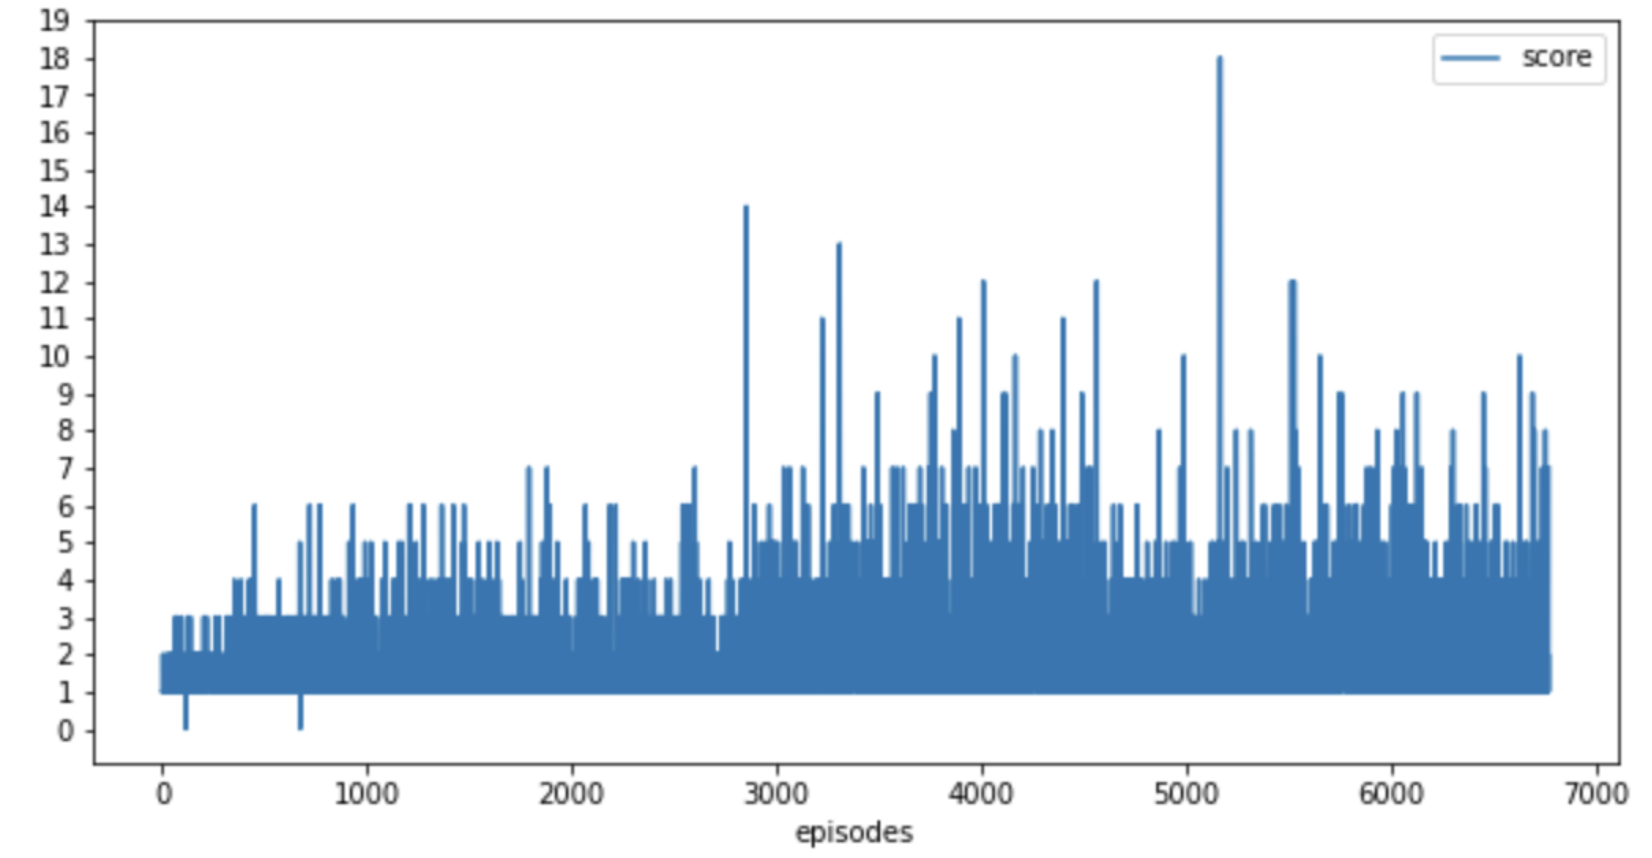
\includegraphics[width=0.5\textwidth]{ForthAgent.png}
% \end{figure}

% \subsubsection{Conclusion}
% Based on the result, we noticed that there is improvements compared with other agents. However, we still have concerns. This agent changed not only  image processing but also the reward function settings. Thus, we could not be able to say that we have found a clear direction for future parameter tuning. 

\section{Current Problems and Future Improvement}

\subsection{Accuracy of Object Detection}
Also, in our experimental agent, we might have found a better way to pre-process images for our CNN model. There are still improvement that we could work on. In the below image processed by the edge detection, we noticed that not only the edge of objects are highlighted, but also the edge of shadow. This may negatively affect the accuracy of our CNN model. Our model seems to perform poorly since the image input is too complicate. It makes q value from the model has very high variance, and it affect our bellman's equation does not work. Therefore, we are first trying to normalize the q value before updating the new value, and we are working on figuring out the actual impact of the edge of the shadow in our model and if there is solution for this problem.

\subsection{Latency Between State Changing and Decision Making}
We also found a serious problem that have negative impact the performance of our agent while this problem does not related neither the reward function setting and the accuracy of our CNN model. Due to the limitation of our computing power, there may be a huge latency between getting output from the model and feeding the state of game to it. However, during the computing process, the game state is still changing. So, if our agent is on the road with a car running to it, it can be terminated by the car before it gets the result from the model. There are two potential solutions. Firstly, we can add a pasue function in the game, so when we freeze the game to maintain the state as same as the one we feed to the model. Second, we can first calculate the frame rate of the game, which can give us a time limit for computing, so our agent get the output from the model on time. 

\subsection{Efficiency Improvement}
Since our model needs massive amount time to observe the game, and trains several agents with different parameters in order to optimize the result, we need to find ways that can accelerate the training process. However, most of our team members are using laptops that the computation power is limited. Therefore, the ideal solution is to migrate our project into cloud. We have tried the google CoLab, but the time it takes too much time to read data from the Google driver, which results the restricted performance. Our next step is to try the GCP AI platform, where we will pack everything into a bucket and upload it to the cloud server, and then utilize various processors that are designed for accelerating deep learning. Hopefully, with the help from Cloud, we can find the most optimized parameter as soon as possible. 

% \bibliographystyle{plain}
% \bibliography{references}
\end{document}
